\begin{enumerate}

\item[a)] Se inicializan las variables globales proximaA y proximaB (que se usaran para indicar el indice de la proxima tarea del jugador) en 0, jugadorJugando en 0, actual (que sera el indice de la tarea que esta corriendo, será 0-8), y gdt_tss_actual en 13 (la entrada 14 corresponde a la idle y de ahi en adelante a las tareas del jugador 1 y 2).

\item[b)] En este apartado nos tomamos ciertas libertas con respecto a la organización de las funciones del scheduler, a continuación detallaremos el uso de cada una. La función {\tt sched\_proxima\_a\_ejecutar} es renombrada como {\tt sched\_proximo\_indice}. Esta llama a {\tt obtener\_proxima\_viva} la cual hace los chequeos de jugadorJugando (si el jugadorJugando es 0, osea el jugador 1, buscará una tarea viva del otro jugador, y viceversa), en caso de encontrar una tarea viva del otro jugador, actualiza jugadorJugando a dicho jugador y devuelve el indice de la tarea, en caso de no encontrar una tarea viva devuelve {\tt 0xff}. El resultado de {\tt obtener\_proxima\_viva} se lo compara con {\tt 0xff} y en ese caso se llama a {\tt pasar\_a\_idle} y se retorna {\tt 0xff}. En caso contrario, se llama a {\tt cambiar\_tarea} con la proxima tarea viva, se actualiza el clock de la tarea en el mapa y se devuelve el indice en la GDT de la tss de la tarea a la que se pasa.

El funcionamiento {\tt pasar\_a\_idle} pasa por revisar si actual es {\tt 0xff} y en ese retorna  {\tt 0xff} terminando con la ejecución (dado que la idle no debe ser capaz de hacer un cambio de tarea a si misma). En caso contrario, se llama a {\tt cambiar\_tarea} con {\tt 0xff} y se retorna el indice en la GDT de la TSS de la tarea IDLE.

El cambio de tarea realizado por {\tt cambiar\_tarea} consta de comprobar si el parametro tomado es igual a {\tt 0xff} y en ese caso se modifica actual con este valor y gdt_tss_actual pasa a ser 1 (luego con un calculo de $gdt$_$tss$_$actual + 13$ $<<$ 3 en {\tt sched\_proximo\_indice} se obtendría el indice de la tss en la GDT). En caso contrario, actual pasa a ser igual al parámetro tomado por la función se resetean proximaA y proximaB según corresponda, en caso de superar el número de tareas (en caso de ser mayor a 8 vuelve a 0). Por último se obtiene el índice de la tss de la tarea actual en la GDT y se lo asigna a gdt_tss_actual.

\item[d)] Se modifica la rutina de atención de la interrupción {\tt 0x46} para que luego de llamar a {\tt game\_syscall\_manejar} desaloje a la tarea que la llamo mediante los siguientes pasos: se llama a {\tt pasar\_a\_idle} y un jmp far al selector que devuelve esta, con el offset 0.

\item[e)] La rutina de atención se modifica para que ejecute los siguientes pasos, permitiendo el intercambio de tareas por cada ciclo de clock:
   \begin{itemize}
	\item Se guarda en un registro el resultado obtenido en {\tt sched_proximo_indice}
	\item Se lo compara con {\tt 0xff}, valor que usamos para identificar a la tarea idle. En este caso, indica que no quedan piratas vivos para ejecutar. De ser iguales no se produce salto alguno.
	\item Se lo compara con el valor previo del selector, si son iguales quiere decir que es la única tarea activa. Como una tarea no debería ser capaz de saltar a si misma, no se produce salto alguno y continúa corriendo la tarea.
	\item Si ninguno de los 2 casos anteriores se cumple, se procede a ejecutar un JMP FAR al resultado de realizar {\tt sched_proximo_indice}, al offset correspondiente en la GDT a la tss de la tarea destino.
	\end{itemize}
	
\item[f)] Para manejar el hecho de desalojar una tarea cuando esta produce una excepción implementamos, en cada rutina de atención de excepciones, un llamado a la función {\tt game\_matar\_pirata\_interrupt}. Esta función, por un lado llama a la función {\tt game\_matar\_pirata} la cuál se encarga de hacer lo relacionado con mostrar el clock del pirata como muerto y setear en 0 el atributo vivo del pirata, de manera que no se puedan producir saltos a esta tarea. Por otro lado, revisa si había algun minero pendiente en el arreglo de mineros pendientes del jugador en cuestión, de ser así lo lanza con la posición del botín previamente almacenada en dicho arreglo y actualiza sus valores.

\item[g)] El modo debug permite capturar y mostrar por pantalla las excepciones causadas por la operación de los piratas. El mismo se activa presionando la tecla Y del teclado. Una vez activo, el juego continúa de manera normal, esperando a que se produzca la próxima excepción por parte de una tarea cualquiera. Cuando esto suceda, se mostrará un cuadro con la información correspondiente a la tarea que experimentó la falla como se muestra en la siguiente figura.

\begin{figure}
  \centering
    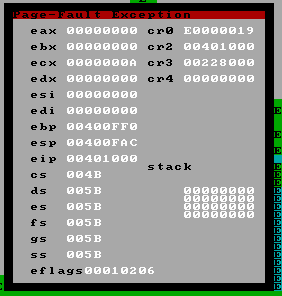
\includegraphics{imagenes/debug.png}
  \caption{Ventana debug}
  \label{fig:ejemplo}
\end{figure}
 \FloatBarrier
 
Al presionarse nuevamente la tecla Y, el cuadro de debug desaparece, pudiendo continuarse con el juego, siempre a la espera de la próxima excepción.
En la pantalla se muestra la representación hexadecimal del estado de los registros eax, ebx, ecx, edx, esi, edi, ebp, esp, eip, cs, ds, es, fs, gs, ss, cr0, cr2, cr3 y cr4. Además, mostramos la representación del registo eflags y de los 4 valores superiores de la pila, también en hexadecimal.
Para regular este modo, tomamos la decisión de crear una variable global debug que posee 3 estados distintos: (0) para debug no activado, (1) para debug activado, (2) para modo mostrando. Al iniciar el juego esta variable se setea en 0, el pasaje a 1 se regula por la atención de teclado, al apretar la tecla correspondiente, y el pasaje al modo 2 se realiza al capturar la primer expepción que ocurra luego de pasar a modo 1.
En el caso de estar mostrando y presionar la tecla Y, se restaurará la pantalla y se continuará con el juego. Para restaurar la pantalla, almacenamos previamente el estado de la pantalla en el sector ocupado por la ventana de debug en un buffer. Este buffer se encuentra en el área de memoria libre a la que denominamos {\tt VideoCache}.
Modificamos las rutinas de atención de las excepciones, agregando las lineas necesarias para, si el modo debug se encontraba activado, llamar a la función {\tt screen\_muestra\_error} luego de matar a la tarea que produjo el error. Esta función se encarga de copiar al buffer de video el sector de la pantalla que se verá modificado y muestra la ventana con la información exigida y setea la variable {\tt debug} en 2 para indicar que se encuentra mostrando.
A la función {\tt screen\_muestra\_error} previamente mencionada, se le pasan por parámetro los valores de los registros, y otros valores a mostrar. Ya dentro de la función,  y despues de copiar la pantalla, obtenemos los valores de los registros (cr0, cr2, cr3, cr4).
Mientras el cuadro se encuentra en pantalla, la función {\tt obtener\_proxima\_viva} del scheduler devuelve siempre el valor {\tt 0xFF}, indicando que la ejecución debe quedarse en la tarea \textit{Idle}. Dicho comportamiento se conserva hasta que se presiona la tecla Y, con la cual se reanuda el juego. Además, vale aclarar que desde la rutina de atención del teclado, se realizan las comparaciones necesarias sobre la variable debug para que no suceda evento alguno (no se podrán lanzar nuevas tareas), salvo que se presione la tecla Y reanudando el juego.


\end{enumerate}
